\documentclass{lecturenotes}

\renewcommand{\vecka}{15}
\newcommand{\tema}{Avslutning, Utblick}

\setbeamertemplate{footline}[frame number]
\title[Föreläsningsanteckningar EDA016, 2015]{EDA016 Programmeringsteknik för D}
\subtitle{Läsvecka \vecka: \tema}
\author{Björn Regnell}
\institute{Datavetenskap, LTH}
\date{Lp1-2, HT 2015}

%%%%%%%%%%%%%%%%%%%%%%%%%%%%%%%%%%%%%%

\begin{document}

\frame{\titlepage}
\setnextsection{\vecka}
\section[Vecka \vecka: \tema]{\tema}
\frame{\tableofcontents}

\subsection{Att göra denna vecka}
\begin{Slide}{Att göra i Vecka \vecka: Repetition, uppsamling, tentaplugg.}
\begin{enumerate}
\item Uppsamling: \Alert{gör klart och redovisa kvarvarande labbar och inlämningsuppg. på veckans resurstider}
\item Träffas i samarbetsgruppen \& hjälp varandra att tentaplugga.
\item Ingen labbtid denna vecka - använd resurstider för uppsamling och frågor inför tentapluggande.
\item Kolla på tentapluggtipsen på \href{https://github.com/bjornregnell/lth-eda016-2015/blob/master/lectures/notes/week14.pdf}{förra föreläsningen}.
\end{enumerate}
\end{Slide}

\subsection{Om tentamen}

\begin{Slide}{Extenta: Fortsättning på genomgång av Sociala-nätverkstentan}
\begin{itemize}
\item Tenta: \href{http://fileadmin.cs.lth.se/cs//Education/grundkurs/extentor/150318.pdf}{150318.pdf}
\item Lösning: \href{http://fileadmin.cs.lth.se/cs//Education/grundkurs/extentor/sol-150318.pdf}{sol-150318.pdf}
\end{itemize}
Frågor på uppgift 1-3? \newline \\ \pause
\scriptsize \Emph{Uppgift 4}:  
Antag att det sociala nätverket i föregående uppgift ska vidareutvecklas för att stödja en ny typ av användare. Man vill nu att både företag och privatpersoner ska kunna använda nätverket och man vill lägga till detta utan att ändra i någon av klasserna i tidigare uppgifter. Företag ska, förutom namn, id, aktiviteter och vänlista (som en ''vanlig'' \code{User} har) även ha organisationsnummer och slogan. Vi gör förändringen genom att införa en ny klass.
\\
\begin{enumerate}[a.] %Kanske var vi någon egen typ för det här...hittade inte.
\item Beskriv hur förändringen bäst kan införas i det projekt som beskrivs i tentan. En korrekt förklaring ger 2 poäng.
\item Skriv kod för att visa hur den nya klassen ser ut. Lösningen behöver inte innehålla några andra metoder förutom konstruktorn. Korrekt kod ger ytterligare 3 poäng.
\end{enumerate}

\end{Slide}

\begin{Slide}{Tenta: anmälning och anonyma tentor}
\begin{itemize}
\item Du \Alert{måste vara godkänd} på \Alert{alla} labbar + inlämningsuppg. för att få tenta.
\item Läs \Alert{alla} instruktioner \Alert{noga} och \Alert{anmäl dig} här: \\ \url{http://www.student.lth.se/studieinformation/anonyma-tentor/}
\item \Emph{Gruppbonus}: Din grupps samarbetsbonus meddelas via mejl. Kontakta mig om något verkar felaktigt. 
\end{itemize}
\end{Slide}

\subsection{Inlämningsuppgift}
\begin{Slide}{Inlämningsuppgift Bank; diskussion + utblick}
\Emph{Exempel på klurighet} \\
Specifikationen tillåter uttag som är större än saldot på kontot, men i det textuella användargränssnittet ska felmeddelande ges vid för stora uttag som inte medges. \\ 
\vspace {1em} Hur löser vi det? \\
\pause Genom att implementera logik som förhindrar för stora uttag.
 \\ \vspace {1em} 
 \pause
\begin{itemize}
\item När man använder ett api behöver man förstå vad api:et omfattar och hur det är tänkt att användas. 
\begin{itemize}
\item Vad behöver jag själv kolla? 
\item Vad kollas av koden i api:et som jag använder? 
\item Vilken klass ansvarar för vad?
\end{itemize}
\item Mer om design-frågor i OMD-kursen.
\end{itemize}
\end{Slide}

\begin{Slide}{Inlämningsuppgift Draw; diskussion + utblick}\footnotesize
\Emph{Exempel på klurighet} \\
Utvidgning: relativ förflyttning med tangentbordet. \\Men klassen \code{se.lth.cs.pt.shapes.Shape} har inga metoder som exponerar attributen \code{x} och \code{y}.\\ 
\vspace {1em} Hur löser vi det? 
\pause Två olika lösningar:
\begin{itemize}\footnotesize
\item Kopiera  \code{se.lth.cs.pt.shapes.Shapes} till mitt eget paket och lägg till metoderna \code{getX()}, \code{getY()} eller \code{deltaMove(dx, dy)}
\item Eftersom attributen \code{x} och \code{y} är \code{protected} i \code{Shape} så kan vi med en ny klass \code{LocatableShape extends Shape} och implementera \code{getX()}, \code{getY()} eller \code{deltaMove(dx, dy)} i denna
\end{itemize}
 \pause \vspace{1em} Viktiga generella observationer:
\begin{itemize}\footnotesize
\item Om du har tillgång till källkoden och får kopiera den kan du bygga vidare på koden (en s.k. \href{https://sv.wikipedia.org/wiki/Fork}{fork}), men vad göra om api:et kommer i ny version? 
\item Genom arv kanske det går att fixa det du saknar, men vad göra om api:et kommer i ny version?
\end{itemize}
\end{Slide}

\subsection{Kursutvärdering}
\begin{Slide}{CEQ -- Course Experience Questionnaire}\footnotesize
\begin{itemize}
\item Görs på hela LTH på samma sätt. Alla får länkar via mejl.
\item Snälla fyll i CEQ! Jag är \Alert{mycket tacksam} för all konstruktiv feedback! \\ Hög svarsfrekvens är viktigt för att kunna dra slutsatser om variationen i svaren och signifikansen i sammanställningen.
\item Del 1: Generella påståenden, alla med 5-gradig skala: \\ tar helt avstånd ... instämmer helt
\item Del 2: \Emph{Fritextfrågor}: \\
''Vad  tycker  du  var  det  bästa  med  den här  kursen?'' \\
''Vad  tycker  du  främst  behöver  förbättras?''
\item Fördel med CEQ: Samma alla kurser alla år medger jämförelse över tid.
\item Begränsning med CEQ: Saknar frågor kopplat till specifika kursmoment.
\item Mer om CEQ här: \url{https://www.ceq.lth.se/}
\end{itemize}
\end{Slide}

\begin{Slide}{Kursspecifik utvärdering om specifika kursmoment}
\begin{itemize}
\item Jag vill gärna att alla gör den LTH-gemensamma, anonyma kursutvärderingsenkäten \href{https://www.ceq.lth.se/}{CEQ}. Dina fritext-kommentarer om vad som är det bästa med kursen och vad som främst behöver förbättra emottages mycket tacksamt i CEQ-utvärderingen!
\item Jag vill också komplettera CEQ med en kursspecifik utvärdering av specifika kursmoment i denna kurs och jag är därför \Alert{mycket tacksam} om alla fyller i denna snarast: \\ \url{http://goo.gl/forms/x5ClcMX22Q}
\item Jag behandlar dina svar konfidentiellt, men ber om din STiL-id så att jag kan återkomma om jag mot förmodan undrar något mer.
\item Din input är mycket värdefull vid framtida kursutveckling!
\end{itemize}
\end{Slide}

\subsection{Grumligtlådan}
\begin{Slide}{Några avslutande lappar ur Grumligtlådan}
\begin{itemize}
\item \Emph{overloading}: flera metoder med samma namn
\item \Emph{override}: ersätta metod i subklass
\item \Emph{iterator}: ett objekt med metoder för att iterera över elementen i en samling
\item ''När du säger \Emph{Java} exakt vad menar du då?''
\begin{enumerate}\footnotesize
\item Ett programspråk
\item En virtuell maskin och exekveringsplattform
\item En stor uppsättning standardbibliotek med färdiga klasser
\item En global gemenskap kring ett stort antal öppen-källkodsbibliotek
\end{enumerate}
\item \Emph{volatile}: speciellt nyckelord för skydd mot samtidig access av gemensamma variabler i jämlöpande trådar. \\ \footnotesize Java har speciella språkkonstruktioner och bibliotek för att hantera trådar som exekverar samtidigt. Detta är ett avancerat och intressant område som ni läser mer om i realtidsprogrammering.
\end{itemize}
\end{Slide}

\Subsection{Utblick}

\begin{Slide}{Utblick: Vart är Java och JVM-teknologin på väg?}\footnotesize
\begin{itemize}
\item En viktig trend är kombinationen av objekt-orientering och funktionsprogrammering och detta visar sig i \href{http://www.oracle.com/technetwork/java/javase/8-whats-new-2157071.html}{Java 8} med sina anonyma funktioner (s.k. lambda expressions) och nya samlingen java.util.stream.
\item I \href{http://www.javaworld.com/article/2984263/java-platform/oracle-says-java-9-modules-will-be-a-boon-for-developers.html}{Java 9} som resultat av ''\href{http://www.infoworld.com/article/2895889/java/oracle-java-9-future-lego-like.html}{Project Jigsaw}'' kommer mycket handla om modularisering av JDK som möjliggör skräddarsydda, mindre runtime-versioner av JVM.	
\item Mycket av utmaningarna handlar om att dra nytta av många kärnor och parallellprogrammering blir allt hetare. Därför jobbar man mer och mer med oföränderlig data som gör det lättare att dela upp beräkningar på flera kärnor.
\item Det finns flera livaktiga språk som kör på JVM, t.ex.  \href{https://sv.wikipedia.org/wiki/Scala\_\%28programspr\%C3\%A5k\%29}{Scala} och  \href{https://sv.wikipedia.org/wiki/Clojure}{Clojure} men också \href{https://sv.wikipedia.org/wiki/Javascript}{Javascript} med skriptmotorn \href{https://en.wikipedia.org/wiki/Nashorn\_\%28JavaScript_engine\%29}{Nashorn} 
\item Med kompilatorn för Scala till Javascript \href{http://www.scala-js.org/}{Scala.js} kan man dela kod mellan en server som kör på JVM och en klient som kör i webbläsaren.
\end{itemize}
\end{Slide}

\begin{Slide}{Utblick: Vart är software engineering  på väg?}
Några faktorer som skapar förändringstryck för ökad produktivitet i utvecklingsprocessen för mjukvara:
\begin{itemize}
\item Snabbast vinner. 
\item Jakt på kompetens. 
\item Sakernas internet.
\end{itemize}
\vspace{1em}
Några starka trender:
\begin{itemize}
\item \href{https://en.wikipedia.org/wiki/Open_source}{Open source}
\item \href{https://en.wikipedia.org/wiki/Big_data}{Big Data}
\item \href{https://en.wikipedia.org/wiki/DevOps}{Devops}
\end{itemize}
\end{Slide}
\Subsection{Frågestund}

\Subsection{Om nästa läsperiod: Gäster Anna Axelsson \& Martin Höst}

\subsection{Avslutning och tack för mig!}
\begin{Slide}{Hoppas att kursen varit kul och lärorik!}

\includegraphics[width=5cm]{img/gurka.jpg}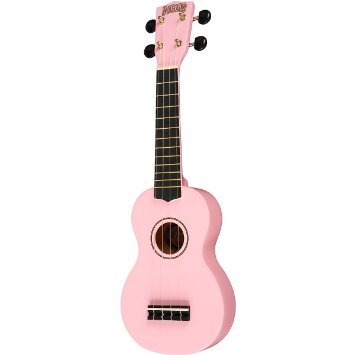
\includegraphics[width=5cm]{img/ukulele.jpg}

\end{Slide}

\begin{Slide}{Ett stort TACK för...}
\begin{itemize}
\item ... att ni kämpat så glatt!
\item ... att ni ställt massor med frågor!
\item ... att det har varit så hög närvaro på föreläsningarna!
\item ... att ni är så konstruktiva och verkligen vill lära er!
\end{itemize}
\vspace{2em} \pause

\Alert{Ett stort LYCKA TILL på vägen till att bli en \\ kompetent och innovativ systemutvecklare!}
\end{Slide}
\end{document}